\begin{figure*}[htbp]
    \centering
    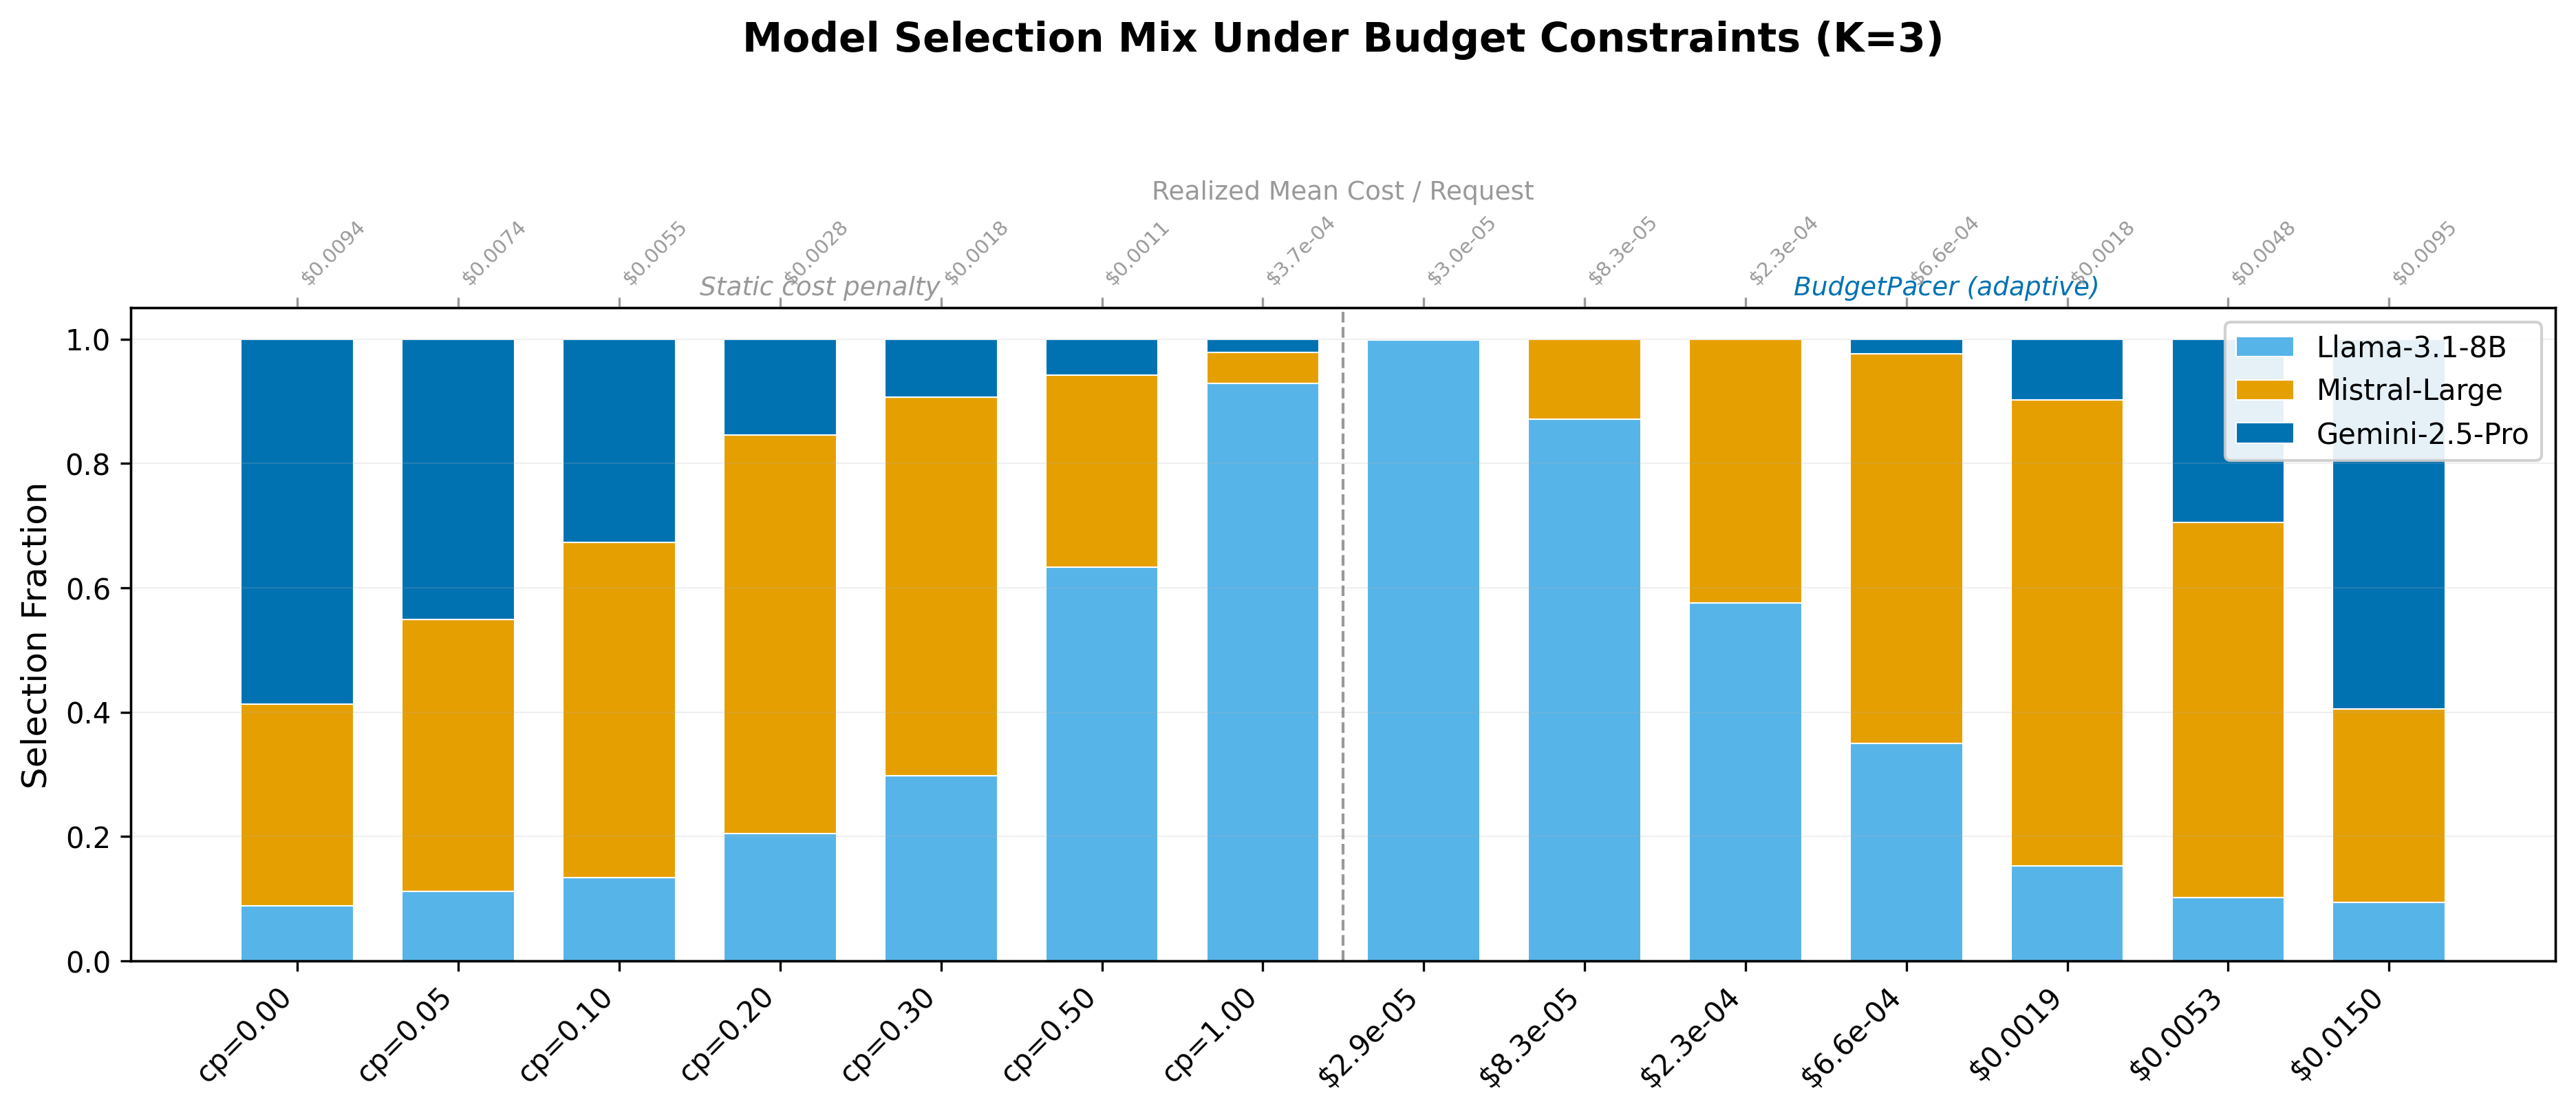
\includegraphics[width=\linewidth]{../experiments/01_stationary_budget_pacing/results/model_mix.pdf}
    \caption{Model selection fractions under the static cost penalty
    (left of dashed divider) and the BudgetPacer (right).
    The top axis shows the realised mean cost per request for each
    condition.  (20~seeds, averaged.)
    %
    \textbf{Static baseline:}  Increasing $\lambda_s$ from $0$ to $1$
    smoothly shifts the mix from Gemini-dominant to
    Llama-dominant, with Mistral peaking
    at intermediate values.
    The transition is gradual because the static penalty is a fixed bias
    in the UCB score; the router must balance this bias against
    contextual reward predictions on every request.
    %
    \textbf{BudgetPacer:}  The transition is sharper and
    budget-compliant by construction.  At tight targets
    ($B \leq \$2.3{\times}10^{-4}$), the hard ceiling excludes Gemini
    entirely and the soft penalty further suppresses Mistral,
    producing a Llama-heavy mix.  At the moderate target
    ($B{=}\$6.6{\times}10^{-4}$) the pacer discovers a
    Llama/Mistral blend that is not reachable by any single
    static $\lambda_s$ value: the nearest static point
    overweights Llama at the expense of quality.
    At loose targets ($B \geq \$0.005$) the pacer converges to the
    unconstrained mix.
    %
    The key qualitative difference is that the static baseline's
    operating point is determined by a dimensionless weight whose
    relationship to dollar cost depends on the specific model portfolio
    and its pricing---a different portfolio requires re-tuning.
    The pacer takes a dollar target directly: ``keep average cost below
    \$X/request'' translates to a single parameter regardless of the
    number of models or their price ratios.
    }
    \label{fig:model_mix_budget}
\end{figure*}
